\chapter{Evaluation} % (fold)
\label{cha:evaluation}

Die ersten Versuche mussten aufgrund des fehlenden Reifendruckes abgebrochen werden. Dies konnte mit einer Luftpumpe behoben werden. Falls die Akkus nicht genug Spannung liefern können, stürzt der Roboter nach wenigen Metern ab.\par
Die erste Rundfahrt wurde ohne funktionstüchtige Akkus durchgeführt. Die Strom\-ver\-sor\-gung wurde mittels zwei Kabeltrommeln gesichert. Des Weiteren wurde immer ein Tisch mit einem Monitor, Maus, Tastatur und Netzteil hinterhergezogen. Durch den Tisch konnte in vielen Räumen nicht gewendet werden. Des Weiteren mussten die Kabel immer aus dem Weg gebracht werden. Dies stellte, wie auch die begrenzte Kabellänge, eine Einschränkung des abgefahrenen Bereiches dar. Viele Räumen konnten aufgrund des begrenzten Platzes und der dort schon vorhandenen Möbel etc. nicht vollständig oder nur ansatzweise kartiert werden. Der Roboter ist aufgrund fehlender Stromquelle zweimal abgestürzt, da das Kabel nicht lang genug war oder hängengeblieben ist.\par
Die vor den Abstürzen aufgenomenen Nachrichten konnten zu zwei Karten zusammengesetzt werden. Die beiden Karten wurden anschließend mit einem Bildbearbeitungsprogramm zusammengesetzt (siehe Abbildung \ref{fig:vollstaendige-karte}).\par

\begin{figure}[H]
	\centering
	
\includegraphics[width=14cm]{a-1.png}
	\caption{Vollständige Karte}
	\label{fig:vollstaendige-karte}
\end{figure}

Mit dem Einbau eines neuen Akkus konnte eine weiter Kartierungsfahrt durchgeführt werden. Da auf den Einsatz der Kabbeltrommeln und des Tisches verzichtet wurde, konnte in dieser Fahrt die kartierten Räume besser durchfahren werden.\par
Generell sollte man den Roboter stehts in einer gleichmäßig langsamen Ge\-schwin\-dig\-keit fortbewegen. Außerdem sollte in jedem Fall ein Rückwärtsfahren verhindert werden, da dies die Odometrie des Roboters stören kann. Es können ansonsten während der Kartenerstellung falsch gewinkelte oder plazierte Räume entstehen (siehe Abbildung \ref{fig:fehlgeschlagen}).

\begin{figure}[!htb]
	\centering
	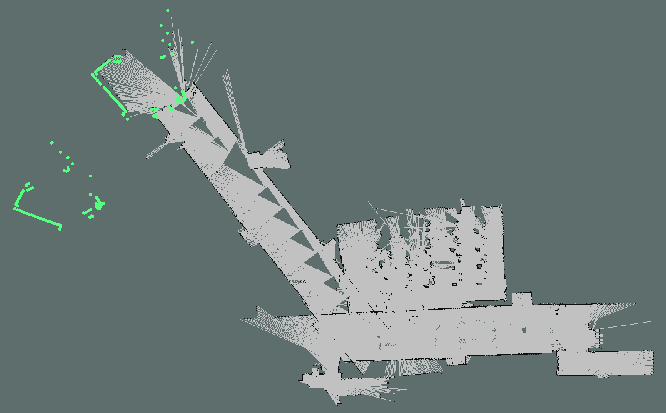
\includegraphics[height=6cm]{fehlgeschlagen.png}
	\caption{Fehlgeschlagene Kartierung}
	\label{fig:fehlgeschlagen}
\end{figure}

Die bei der Durchführung erstellten Karten sind von variabler Qualität. Einige Räume wurden nicht korrekt aneinander ausgerichtet. Im Allgemeinen sind die Grundrisse der kartierten Räume aber immer zu erkennen. Auch ist zu beachten dass der Algorithmus mit den selben Parametern unterschiedliche Karten generieren kann (siehe Abbildung \ref{fig:zweiter-lauf-eins} und Abbildung \ref{fig:zweiter-lauf-zwei}).

\begin{figure}[!htb]
	\centering
	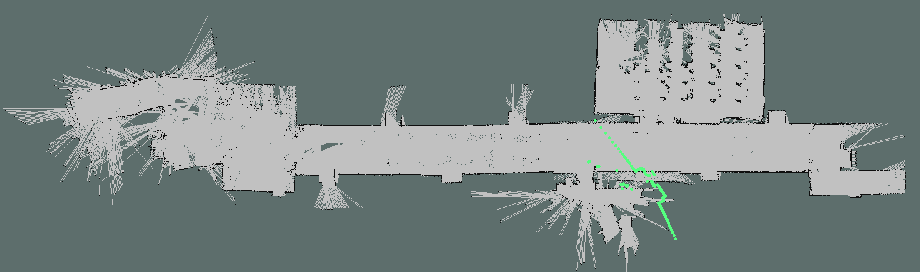
\includegraphics[width=8cm]{zweiter-lauf-eins.png}
	\caption{Karte für die zweite Kartierung}
	\label{fig:zweiter-lauf-eins}
\end{figure}

\begin{figure}[!htb]
	\centering
	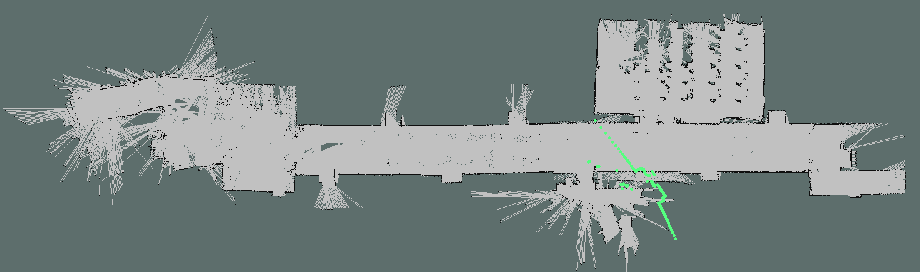
\includegraphics[width=8cm]{zweiter-lauf-eins.png}
	\caption{Karte für die zweite Kartierung}
	\label{fig:zweiter-lauf-zwei}
\end{figure}

% chapter evaluation (end)